%%%%%%%%%%%%%%%%%%%%%%%%%%%%%%%%%%%%%%%%%%%%%%%%%%%%%%%%%%%%%%%%%%%%%%%%
\chapter{Introduction}
\label{chapter:introduction}
%%%%%%%%%%%%%%%%%%%%%%%%%%%%%%%%%%%%%%%%%%%%%%%%%%%%%%%%%%%%%%%%%%%%%%%%
\localtableofcontents

%%%%%%%%%%%%%%%%%%%%%%%%%%%%%%%%%%%%%%%%%%%%%%%%%%%%%%%%%%%%%%%%%%%%%%%%%%%%%%%
\section{Context \& Motivation}
\label{section:ch1-context_and_motivation}
%%%%%%%%%%%%%%%%%%%%%%%%%%%%%%%%%%%%%%%%%%%%%%%%%%%%%%%%%%%%%%%%%%%%%%%%%%%%%%%

%%%%%%%%%%%%%%%%%%%%%%%%%%%%%%%%%%%%%%%%%%%%%%%%%%%%%%%%%%%%%%%%%%%%%%%%%%%%%%%
\subsection{Context}
\label{subsection:ch1-context}
%%%%%%%%%%%%%%%%%%%%%%%%%%%%%%%%%%%%%%%%%%%%%%%%%%%%%%%%%%%%%%%%%%%%%%%%%%%%%%%

With the surge in data collection and computing resources over the last 20 years, the interest and use cases for Machine Learning have grown exponentially.
More specifically, Deep Learning, a subfield of Machine Learning, consisting of training Deep Neural Networks on high-level
data (images, sounds, texts) have shown great achievements.
In recent years, Deep Neural Networks achieve state-of-the-art performances in a variety of domains such as image recognition~\cite{lecun1998gradient,krizhevsky2012imagenet,He_2016_CVPR,tan2019efficientnet}, object detection~\cite{redmon2016you,liu2016ssd,redmon2017yolo9000}, natural language processing~\cite{merity2016pointer,radford2018Language,brown2020language}, speech recognition~\cite{hinton2012deep,abdel2014convolutional,yu2016automatic}, etc.

\begin{figure}[t]
  \centering
  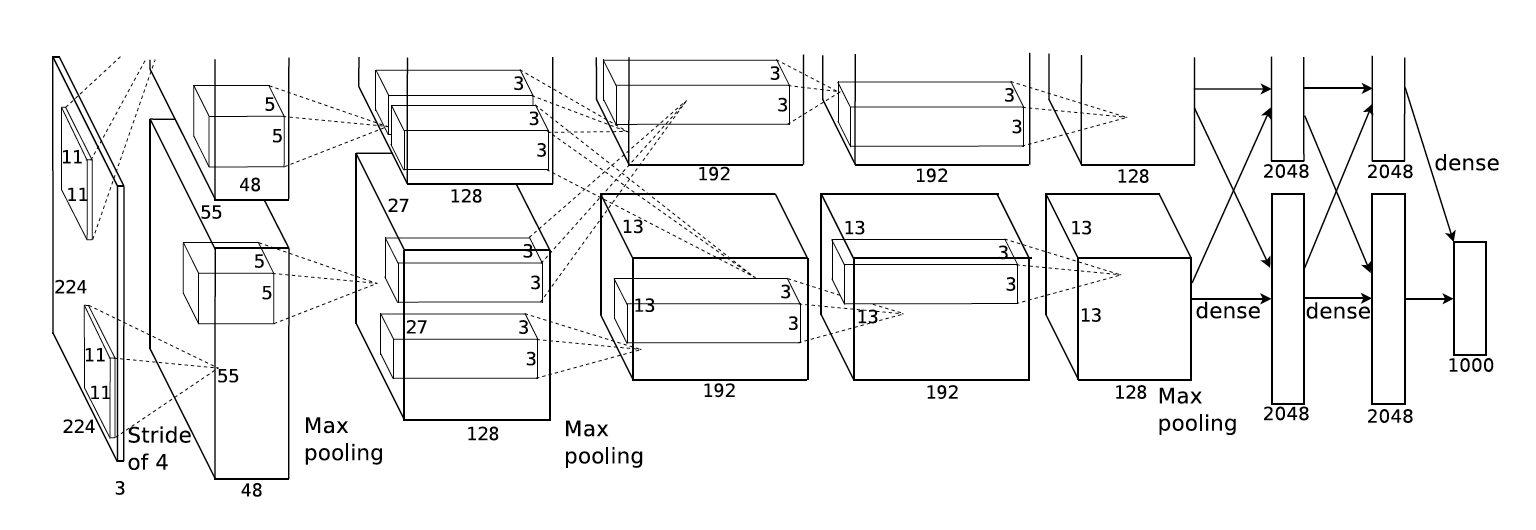
\includegraphics[scale=0.2]{figures/chapter1/alexnet.png}
  \caption{This figure shows the neural network architecture (AlexNet) proposed by~\citet{krizhevsky2012imagenet} which won the ImageNet Large-Scale Visual Recognition Challenge in 2012.}
  \label{figure:ch1-alexnet_network}
\end{figure}

One of the first breakthroughs of Deep Learning was during the 2012 ImageNet Large-Scale Visual Recognition Challenge~\cite{ILSVRC15} which consists of evaluating algorithms for object detection and image classification.
In this challenge, \citet{krizhevsky2012imagenet} achieved \nth{1} place and beat every other participants by a 10.8\% margin with a neural network architecture called \emph{AlexNet} (see Figure~\ref{figure:ch1-alexnet_network}). 
The main reasons for such performance are three fold: first, they used a network architecture with more than 60 million parameters which was significant for the computational resources of the time; they used the ImageNet database~\cite{imagenet_cvpr09} which consists of 1.2 million labeled images with 1000 different classes for training their network; finally, they used graphics processing units (GPUs) to speed up the mathematical operations, reducing training time from several months to just a few days. 

\begin{table}[t]
  \centering
    {\small
    \begin{tabular}{llcc}
      \textbf{Computer Vision Models} & & & \\
      \toprule
      Authors & Models & \#Params & TOP-5 Acc. \\
      \midrule
      \citet{krizhevsky2012imagenet} & AlexNet~ & 61M & 84.7\% \\
      \citet{simonyan2014very} & VGG & 144M & 92.0\% \\
      \citet{he2016deep} & ResNet-152 & 60M & 93.8\% \\
      \citet{szegedy2017inception} & Inception-ResNet-v2 & 56M & 95.1\% \\
      \citet{xie2017aggregated} & ResNeXt-101 & 84M & 95.6\% \\
      \citet{hu2018squeeze} & SENet & 146M & 96.2\% \\
      \citet{huang2019gpipe} & GPipe & 556M & 97.0\% \\
      \bottomrule \\
      \textbf{Natural Language Processing Models} & & & \\
      \toprule
      Authors & Models & \#Params & Score \\
      \midrule
      \citet{peters2018deep} & ELMo & 94M & xxx \\
      \citet{radford2018improving} & GPT & 110M & xxx \\
      \citet{devlin2019bert} & BERT & 340M & xxx \\
      \citet{radford2019language} & GPT-2 & 1.5B & xxx \\
      \citet{shoeybi2019megatron} & MegatronLM & 8.3B & xxx \\
      \citet{rosset2020turingnlg} & T-NLG & 17B & xxx \\
      \citet{brown2020language} & GPT-3 & 175B & xxx \\
      \bottomrule
    \end{tabular}
    }
    \caption{The first table shows different networks trained for computer vision with their number of parameters and accuracy that came up in the years after AlexNet. This second table shows different networks trained for Natural Language Processing tasks that came out in the last three years.}
  \label{table:ch1-networks_parameters}
\end{table}

Since this result, many different architectures came out, with more and more parameters leading some years later to near perfect accuracy on the ImageNet Dataset and Computer Vision task in general.
Table~\ref{table:ch1-networks_parameters} shows the different architectures that came out in the years after AlexNet.
While most new architectures have been proposed based on intuition and test and learn approaches, recent research \cite{tan2019efficientnet,rosenfeld2020a} have examined the relationship between the number of parameters (model size), the size of the dataset and the accuracy.
For computer vision models, \citet{tan2019efficientnet} have shown that the relation between model size and accuracy seems to obey a power law. 
This discovery leads them to propose an efficient neural network with similar or higher accuracy than existing ones.  
For Natural Language Processing (NLP) neural networks, this relationship has also been observed and given the availability of large-scale datasets (Common Crawl dataset~\cite{raffel2019exploring} constitutes nearly a trillion words), researchers have been able to scale their models culminating in the 175 billion parameters GPT-3 model proposed by~\citet{brown2020language}. 

As a result, higher performing models in computer vision and natural language processing have enabled the deployment and use of these models in real-world applications such as autonomous vehicles~\cite{fagnant2015preparing}, translation~\cite{wu2016google}, vocal assistants~\cite{li2017acoustic}.
Translation and voice assistants are now used by millions of people around the world and the autonomous vehicles could reshape the transportation industry over the next decade.


%%%%%%%%%%%%%%%%%%%%%%%%%%%%%%%%%%%%%%%%%%%%%%%%%%%%%%%%%%%%%%%%%%%%%%%%%%%%%%%
\subsection{Motivation}
\label{subsection:ch1-motivation}
%%%%%%%%%%%%%%%%%%%%%%%%%%%%%%%%%%%%%%%%%%%%%%%%%%%%%%%%%%%%%%%%%%%%%%%%%%%%%%%


In recent years, researchers have searched for networks with higher and higher accuracy in order to build models that can be deployed into real-world applications. 
However, recent finding suggests that the accuracy cannot be the only metric to optimize. 
Neural networks, when implemented in a critical decision process, need to be efficient, secure and interpretable.
Although accurate, large neural networks lack these properties.

\paragraph{Efficient Neural Networks}
With the growing concern over data privacy, methods such as \emph{federated learning} are gaining ground.
Federated learning involves training a model across multiple decentralized devices (\eg, smartphones) with local data sample. 
This avoids the step of centralizing all users' data into one server, thus addressing the issue of data privacy.  
In this setting, the training needs to be performed with limited computational and memory resources. 
More generally, building efficient neural networks can have upside.
Indeed training state-of-the-art models on the ImageNet dataset needs gigabytes of memory and can take several days to train on a single GPU. 
NLP models are even worst, for example, it has been estimated that the GPT-3 model with 175 billion parameters requires 355 years of training on a single GPU and \$4,600,000 to train on a cloud-based compute platform~\cite{li2020overview}.
Thus, building efficient neural networks can reduce training time, cost and allow for faster research and development.


\begin{figure}[htb]
  \centering
  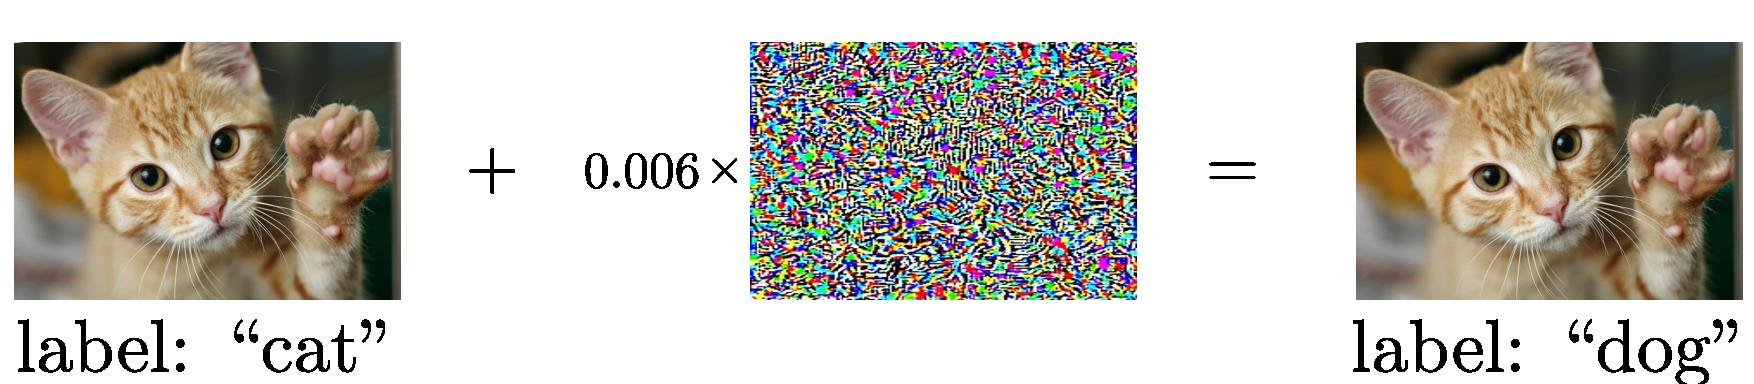
\includegraphics[width=\textwidth]{figures/chapter1/ExampleAdversarialCatDog.pdf}
  \caption{Example of Adversarial Attack on an image. The small perturbation (center) is added to the original image (left) leading to an adversarial image (right).}
  \label{figure:adversarial_image_example}
\end{figure}

\paragraph{Secure and Interpretable Neural Networks}
A mistake by the neural network governing the drive of an autonomous vehicle can lead to injuries or even death, hence a model with perfect accuracy is required.
However, it is difficult to guarantee that no errors will be made.
Having the ability to interpret and understand the error is therefore essential to prevent its recurrence.
Very large neural networks with millions, or more, parameters act as a kind of black box and are difficult to interpret.
Algorithms \cite{lundberg2017unified} for interpreting the decision of a machine learning models scale exponentially with the number of parameters making it impractical for large neural networks. 
Furthermore, large neural networks due to a high complexity and expressivity exhibit instability to small perturbations of their inputs.
The best example of this phenomenon is the vulnerability of neural networks to \emph{adversarial examples}, \ie, imperceptible variations of the natural examples, crafted to deliberately mislead the models~\cite{globerson2006nightmare,biggio2013evasion,Szegedy2013IntriguingPO} (see Figure~\ref{figure:adversarial_image_example}). 
This behavior can cause serious security problems for neural networks used for critical decision-making for example self-driving cars.


%%%%%%%%%%%%%%%%%%%%%%%%%%%%%%%%%%%%%%%%%%%%%%%%%%%%%%%%%%%%%%%%%%%%%%%%%%%%%%%
\section{Problem Setting}
\label{section:ch1-problem_setting}
%%%%%%%%%%%%%%%%%%%%%%%%%%%%%%%%%%%%%%%%%%%%%%%%%%%%%%%%%%%%%%%%%%%%%%%%%%%%%%%

Neural networks, which find their roots in the work of \citet{mcculloch1943logical,rosenblatt1958perceptron}, can be analytically described as a composition of linear functions interlaced with non-linear functions (also called activation functions).
A neural network $f_\Theta : \Rbb^n \rightarrow \Rbb^m$ can be defined as follows:
\begin{equation}
  f_\Theta(\xvec) \triangleq \phi_{\Wmat_p} \circ \rho \circ \phi_{\Wmat_{p-1}} \circ \cdots \circ \phi_{\Wmat_2} \circ \rho \circ \phi_{\Wmat_1}(\xvec)
  \label{equation:neural_network}
\end{equation}
where $p$ corresponds to the \emph{depth} of the network (\ie, the number of layers), the function $\phi_{\Wmat_i}$ is a linear function parameterized by $\Wmat_i$, $\rho$ is a non-linear function and $\Theta \triangleq ( \Wmat_1, \dots, \Wmat_p )$.
The input space $n$ corresponds to the dimension of the data and the output space $m$ corresponds to the number of classes the network has to classify.

This thesis focuses on the concept of \emph{supervised learning} which refers to the notion of learning the parameters of a neural network in order to map an input to an output based on example input-output pairs.
For example, an image (input) associated with its content: label (output).
As we briefly saw in the previous section, accuracy should not be the only metric to optimize when training, developing and deploying neural networks, efficiency and security are also crucial factors to consider.
Hereafter, we review the two problems and some methods currently applied to address them. 

\paragraph{Over-parameterized to Efficient Network Networks}
Neural networks with dense matrices $\Wmat_i$ are called \emph{Fully Connected Neural Networks} because all the neurons from one activation are connected to all the neurons of the following activation.
Fully connected neural networks can have a very large number of parameters.
For example, with the ImageNet Dataset of input dimension $224 \times 224$, a two-layer fully connected neural network will have more than $2.6 \times 10^9$ parameters.
Generally, this type of neural network has been shown to perform poorly certainly due to the search space being too large for the learning procedure.
Moreover, they are computationally expensive which makes them impractical for a number of use cases (smartphones, IoT devices, etc.).
Indeed, instead of using fully connected neural networks, researchers have devised specific linear operations that reduce the number of parameters and have properties adapted for each use case. 
An example of neural networks with specific linear operations are \emph{Convolutional Neural Networks} (CNN)~\cite{lecun1998gradient,krizhevsky2012imagenet,He_2016_CVPR,tan2019efficientnet} which are state-of-the-art for computer vision tasks.
They use specific linear operations (\eg, convolution) which are specific to image processing and use very few parameters.  
A classical linear layer with a dense matrix has $n \times n$ parameters, a convolution layer only has $k \times k$ parameters where $k$ is the kernel size and is usually small (\eg 3 or 5 for classical convolutional layers).


\begin{figure}[t]
   \centering
   \begin{subfigure}[t]{0.24\textwidth}
       \centering
       \begin{equation*}
	  \leftmatrix
	    a &   &   &   \\
	      & b &   &   \\
	      &   & c &   \\
	      &   &   & d
	  \rightmatrix
       \end{equation*}
       \caption*{diagonal}
   \end{subfigure}
   \hfill
   \begin{subfigure}[t]{0.24\textwidth}
       \centering
       \begin{equation*}
	  \leftmatrix
	    a & b & c & d \\
	    e & a & b & c \\
	    f & e & a & b \\
	    d & f & e & a
	  \rightmatrix
       \end{equation*}
       \caption*{Toeplitz}
   \end{subfigure}
   \hfill
   \begin{subfigure}[t]{0.24\textwidth}
       \centering
       \begin{equation*}
	  \leftmatrix
	    ae & af & ag & ah \\
	    be & bf & bg & bh \\
	    ce & cf & cg & ch \\
	    de & df & dg & dh
	  \rightmatrix
       \end{equation*}
       \caption*{Low Rank}
   \end{subfigure}
   \hfill
   \begin{subfigure}[t]{0.24\textwidth}
       \centering
       \begin{equation*}
	  \leftmatrix
	    a & a^2 & a^3 & a^4 \\
	    b & b^2 & b^3 & b^4 \\
	    c & c^2 & c^3 & c^4 \\
	    d & d^2 & d^3 & d^4
	  \rightmatrix
       \end{equation*}
       \caption*{Vandermonde}
   \end{subfigure}
  \caption{Examples of structured matrices.}
  \label{figure:example_structure_matrices}
\end{figure}

Convolutional neural networks are a type of \emph{structured} neural networks because the convolution operation is a matrix multiplication with a structured matrix \ie, matrix that can be represented with less than $n^2$ parameters. 
In addition to offering a more compact representation, the structure of certain matrices can be leveraged to obtain better algorithms for matrix-vector product, thus optimizing memory and computing operations. 
Structured neural networks have been extensively studied in the field of deep learning \cite{moczulski2015acdc,sindhwani2015structured,NIPS2013_5025}.
Figure~\ref{figure:example_structure_matrices} shows different types of structured matrices that can be used for deep learning.
However, it remains unclear whether other types of structure can be beneficial to other types of applications and which structure can provide both accuracy and efficient computation.

The phenomenon, that neural network with a smaller number of parameters, generalizes better has been theoretically justified \cite{vapnik1982estimation}.
More precisely, \citeauthor{vapnik1982estimation} linked the generalization capability of neural networks to their VC-dimension which is a measure of expressivity of the class of functions.
This complexity measure is based on the number of parameters, therefore, reducing the number of parameters leads to a smaller VC-Dimension, which could lead to better generalizations.



\paragraph{Robust Neural Networks}

The instability of neural networks to small input perturbations has led them to be vulnerable to \emph{adversarial examples}, \ie, imperceptible variations of the natural examples, crafted to deliberately mislead the models.
The study of security properties of learning algorithms is a research field known as \emph{adversarial machine learning} which dates back to 2004 \cite{dalvi2004adversarial}.
More recently, the work of \citet{Szegedy2013IntriguingPO} has bought considerable attention to adversarial examples in the context of Deep Learning.
Since then, a torrent of work has been published in designing attacks and defenses \cite{Szegedy2013IntriguingPO,goodfellow2014explaining,papernot2016limitations,madry2018towards,carlini2017towards,pinot2019theoretical}.


\emph{Adversarial Training}, one of the first effective methods, was introduced by \citet{goodfellow2014explaining} and later improved by \citet{madry2018towards}.
% One of the first effective method is called \emph{Adversarial Training}.
% It was introduced by \citet{goodfellow2014explaining} and later improved by \citet{madry2018towards}.
It consists of augmenting training batches with adversarial examples generated during the training procedure.
By \emph{seeing} adversarial examples correctly labeled during the training procedure, neural networks exhibit increased robustness during the inference phase.
More recently, a new method \cite{farnia2018generalizable} based on the regularization of the Lipschitz constant of the network has been proposed.
In this work, the authors linked the generalization capabilities of neural networks trained with Adversarial Training to their Lipschitz constant; therefore, a reduced Lipschitz constant could lead to a better generalization.



%%%%%%%%%%%%%%%%%%%%%%%%%%%%%%%%%%%%%%%%%%%%%%%%%%%%%%%%%%%%%%%%%%%%%%%%%%%%%%%
\section{Main contributions and Outline of the Thesis}
\label{section:ch1-main_contributions_and_outline_of_the_thesis}
%%%%%%%%%%%%%%%%%%%%%%%%%%%%%%%%%%%%%%%%%%%%%%%%%%%%%%%%%%%%%%%%%%%%%%%%%%%%%%%


% In this thesis, we leverage the properties of \emph{structured matrices} for the problems mentioned in Section~\ref{subsection:ch1-introducing_structured_into_the_architecture_of_neural_networks} and \ref{subsection:ch1-introducing_structured_into_the_learning_procedure}.
%
% More specifically, we study the properties of structured matrices from the Toeplitz family to make two contributions presented below:

In this thesis, we leverage the properties of structured matrices from the Toeplitz family to make contributions in the field of deep neural networks.
More precisely, we focus on building efficient and robust neural networks. 

This thesis is organized in two parts.
First, we use circulant matrices, which are a particular case of Toeplitz matrices, to devise a new compact architecture replacing Fully Connected Neural Networks.
More precisely, we study deep diagonal circulant neural networks, which are deep neural networks in which weight matrices are the product of diagonal and circulant ones.
Besides making a theoretical analysis of their expressivity, we introduce principled techniques for training these models: we devise an initialization scheme and propose a smart use of non-linearity functions in order to train deep diagonal circulant networks. 
Furthermore, we show that these networks outperform recently introduced deep networks with other types of structured layers.
We conduct a thorough experimental study to compare the performance of deep diagonal circulant networks with state-of-the-art models based on structured matrices and with dense models.
We show that our models achieve better accuracy than other structured approaches while requiring 2x fewer weights than the next best approach.
Finally, we train compact and accurate deep diagonal circulant networks on a real-world video classification dataset with over 3.8 million training examples. 

In the second part of this thesis, we leveraged the properties of the structure of convolution to devise a new upper bound on the largest singular value of convolution layers that is both tight and easy to compute. 
Our work is based on the result \cite{gray2006toeplitz} that an upper bounded on the singular value of Toeplitz matrices can be computed from the inverse Fourier transform of the characteristic sequence of these matrices.
From our analysis immediately follows an algorithm for bounding the Lipschitz constant of a convolutional layer, and by extension the Lipschitz constant of the whole network.
Finally, we illustrate our approach on adversarial robustness. 
Recent work has shown that empirical methods such as adversarial training (AT) offer poor generalization~\cite{schmidt2018adversarially}, and can be improved by applying Lipschitz regularization~\cite{farnia2018generalizable}.
To illustrate the benefit of our new method, we train neural networks with Lipschitz regularization and show that it offers a significant improvement over adversarial training alone.





